\RequirePackage{fix-cm}
\documentclass[twocolumn]{svjour3}
\smartqed

\usepackage{fontspec}
\usepackage{xeCJK}
\setmainfont{Times New Roman}
\setCJKmainfont[AutoFakeBold=2,AutoFakeSlant=.2]{SimSun}
\setCJKsansfont{Microsoft YaHei}
\setCJKmonofont{SimSun}
\usepackage{graphicx}
\graphicspath{{../figures/}}
\usepackage{booktabs}
\usepackage{multirow}
\usepackage{threeparttable}
\usepackage{amsmath,amssymb}
\usepackage{microtype}
\usepackage[hidelinks]{hyperref}
\usepackage{xurl}
\usepackage{placeins}

\newcommand{\method}{SRPA-YOLO}
\newcommand{\mapall}{mAP@0.50:\allowbreak0.95}
\newcommand{\srpatablesize}{\footnotesize}
\newcommand{\srpatablesetup}{\srpatablesize\setlength{\tabcolsep}{3.5pt}\renewcommand{\arraystretch}{0.96}}
\renewcommand{\figurename}{图}
\renewcommand{\tablename}{表}
\renewcommand{\refname}{参考文献}
\setlength{\emergencystretch}{2em}
\setcounter{topnumber}{3}
\setcounter{dbltopnumber}{3}
\renewcommand{\topfraction}{0.92}
\renewcommand{\dbltopfraction}{0.92}
\renewcommand{\textfraction}{0.06}
\renewcommand{\floatpagefraction}{0.80}
\renewcommand{\dblfloatpagefraction}{0.80}
\setlength{\textfloatsep}{9pt plus 2pt minus 2pt}
\setlength{\dbltextfloatsep}{8pt plus 2pt minus 2pt}
\journalname{Journal of Real-Time Image Processing}

\begin{document}

\title{SRPA-YOLO：面向实时小型无人机检测的共享表征与私有秩分配方法}
\titlerunning{面向实时小型无人机检测的 SRPA-YOLO}

\author{王显普 \and 职海杰 \and 费庆}
\authorrunning{王显普等}

\institute{王显普 \and 费庆 \at
北京理工大学自动化学院，北京 100081，中国\\
\email{3220252903@bit.edu.cn}\\
\email{feiqing@bit.edu.cn}
\and
职海杰 \at
浙江大学能源工程学院，杭州 310027，中国\\
\email{22427029@zju.edu.cn}
}

\date{收稿日期：待定 / 录用日期：待定}
\maketitle

\begin{abstract}
远距离无人机仅占据少量像素，容易与复杂背景混淆，而机载检测还受到存储和帧时间约束。本文提出共享表征与私有秩分配检测器 SRPA-YOLO，根据分类与定位的任务需求分配预测头容量。模型以 64 通道结构重参数化表征共同支持分类和边界框分布预测，并由零输出初始化的 16 通道表征仅提供加性分类残差，使边界框输出在计算图上直接独立于分类私有表征。部署前，两条 stem 及其任务投影通过代数变换融合为单个 80 通道 $3\times3$ 卷积和一个输出投影，训练期私有路径不会形成并行推理分支。在经图像哈希去重的 DUT Anti-UAV 测试集上，验证集选出的 checkpoint 取得 95.850\% Precision、92.201\% Recall、95.185\% AP@0.50、67.071\% AP@0.50:0.95 和 77.329\% AP@0.75，部署参数量为 2.164 M。相对 YOLOv8n，五项指标分别提高 3.088、8.242、5.057、6.895 和 9.750 个百分点，同时参数量减少 0.842 M。在本文报告的同进程配对协议下，SRPA-YOLO 两轮延迟为 9.7435 和 9.8574 ms，YOLOv8n 对应为 9.8859 和 9.9893 ms。结果表明，在给定硬件与推理设置下，受约束的分类私有容量能够改善精度与紧凑性的权衡，并保持与基线相当的帧时间。
\keywords{无人机 \and 小目标检测 \and 实时图像处理 \and 结构重参数化 \and 知识蒸馏 \and 轻量化检测器}
\end{abstract}

\section{引言}

小型无人机已广泛应用于物流、巡检、应急响应和低空感知，同时也使重点空域产生了稳定、低成本的视觉监测需求。与通用目标检测不同，远距离无人机在缩放后往往不足 $16\times16$ 像素，快速运动、失焦和压缩削弱轮廓，云层、鸟类、建筑和植被又会形成相似响应。检测器既要提高召回率、避免漏警，又要抑制背景误检，并满足边缘平台的存储和延迟约束。现有综述将这种精度与效率矛盾视为视觉反无人机系统的核心问题之一\cite{yasmeen2025review,wang2021smallobjectsurvey}。

YOLO 与 SSD 奠定了单阶段密集预测的实时检测范式\cite{redmon2016yolo,liu2016ssd}，FPN 和 PANet 进一步增强高层语义与浅层空间信息的交换\cite{lin2017fpn,liu2018panet}。FCOS、Focal Loss 与 GFL 分别从无锚预测、类别不平衡和质量感知置信度角度提升密集检测\cite{tian2019fcos,lin2017focal,li2020gfl}。然而，直接增加高分辨率分支或叠加注意力模块会提高显存访问与算子调度开销。EfficientDet、YOLOv4 和 YOLOv7 的实践表明，实际速度取决于骨干、颈部、训练策略和部署图的协同设计，而非仅由 FLOPs 决定\cite{tan2020efficientdet,bochkovskiy2020yolov4,wang2023yolov7}。

本文的出发点是分类与定位并不需要完全相同的特征子空间。分类偏好语义不变性和类间判别性，定位则必须保留对边界和位移敏感的信息。TSD 表明共享候选与表征可能造成任务冲突\cite{wu2020tsd}，TOOD 则说明任务交互需要与任务专属特征及对齐机制并存\cite{feng2021tood}。完整解耦头能够减少直接特征竞争，却会复制代价较高的空间计算；完全共享头更为紧凑，但两项任务受到同一表征预算约束。因此，本文采用受约束的折中方案：保留两任务共用的紧凑基底，仅为分类分配少量附加表征。

基于上述分析，本文提出 Shared-Representation and Private-Rank Allocation YOLO（SRPA-YOLO），作为 YOLOv8 单阶段框架的结构改进，并以 YOLOv8n 为归因精度、参数量与延迟变化的主要基线。模型通过轻量双向颈部保留 P2--P4 特征，每一尺度的检测头包含 64 通道共享 RepConv 和 16 通道分类私有 RepConv。私有输出投影初始化为零，从而保持共享检测器初始的输入--输出函数。部署前采用 RepVGG 的结构重参数化思想\cite{ding2021repvgg}，将两条等效 stem 卷积核沿输出通道拼接，并把任务投影合并为单路径。模型仅在训练期扩展分类容量，推理时不保留并行私有分支。

训练采用两个阶段。阶段 I 利用标准监督、分类响应蒸馏和离散框分布蒸馏学习共享检测器\cite{zheng2022ld}，其中置信度加权项强调可靠的教师定位响应；阶段 II 从函数保持的零残差状态出发，仅优化分类私有 stem 与投影。在该约束下，既有边界框回归函数保持不变，分类获得附加表征容量。本文的方法贡献在于任务专属表征分配、函数保持初始化与精确部署融合的组合；任务解耦、零初始化、蒸馏和结构重参数化本身均已有研究基础。具体贡献如下：
\begin{enumerate}
\item 将预测头容量表述为共享表征与分类私有表征的分配问题。64+16 结构使边界框输出在计算图上直接独立于私有表征，同时允许分类使用共享与私有表征的组合行空间。
\item 构造函数保持的两阶段实现：共享检测器收敛后，从零输出私有投影开始细化，仅增加分类容量，而阶段 II 的边界框回归映射保持固定。
\item 给出精确部署融合公式，将训练期共享/私有路径转换为每尺度一个 $3\times3$ stem 和一个 $1\times1$ 输出层，在浮点舍入误差范围内保持输出，并消除私有分支推理开销。
\item 采用验证集选模、尺度与 IoU 分解、阶段 II 的 40/41/42 匹配随机种子以及同进程配对延迟进行评估。相对 YOLOv8n，最终 checkpoint 的 $P$、$R$、AP@0.50、\mapall{} 和 AP@0.75 分别提高 3.088、8.242、5.057、6.895 和 9.750 个百分点，部署参数量减少 28.0\%。
\end{enumerate}

\section{相关工作}

\subsection{实时与小目标检测}
COCO 评估协议以多个 IoU 阈值上的平均 AP 衡量定位鲁棒性\cite{lin2014coco}。对小目标而言，连续下采样会在形成稳定响应前损失能量和相位信息；高分辨率金字塔虽能补偿，却使计算量随特征面积快速增长。YOLOv8 提供紧凑的无锚实现及可复现训练框架\cite{ultralytics2023}。由于 SRPA-YOLO 在该框架内构建，YOLOv8n 是本文的主结构与部署基线；YOLO11n 作为同期紧凑检测器对照，EDGS-YOLOv8、DRBD-YOLOv8 和 RLRD-YOLO 则用于衡量与 UAV 专用检测器的差异。

硬件友好模块可降低高分辨率特征的代价。MobileNet 使用深度可分离卷积\cite{howard2017mobilenets}，GhostNet 通过廉价变换生成冗余特征\cite{han2020ghostnet}，FasterNet 强调实际 FLOPS 与内存访问的重要性\cite{chen2023fasternet}。本文骨干与颈部沿用 C2f、GhostConv、深度卷积下采样和部分卷积阶段。CBAM 组合通道与空间选择\cite{woo2018cbam}，EMA 以较少参数建模跨空间关系\cite{ouyang2023ema}；这些模块只作为已验证的基础结构保留，并非本文创新点。

\subsection{反无人机基准与专用检测器}
Anti-UAV 系列基准逐步扩展了可见光与红外跟踪条件\cite{zhao2022antiuav,jiang2023antiuav,huang2024antiuav410}。DUT Anti-UAV 检测子集包含大面积复杂背景与极端尺度变化，适合长距离单类 UAV 检测。YOLOv7-GS 针对复杂反无人机背景调整实时检测结构\cite{bo2024yolov7gs}；EDGS-YOLOv8 和 DRBD-YOLOv8 将轻量算子与多尺度增强结合\cite{huang2024edgs,jiang2024drbd}；RLRD-YOLO 强调轻量化与小目标鲁棒性的平衡\cite{li2025rlrd}。

IASL-YOLO 将轻量骨干与自适应特征融合结合，BRA-YOLOv10 则联合多尺度表征与结构化通道剪枝\cite{yang2025iasl,zhang2025brayolo}。二者均通过重新分配骨干或特征金字塔中的计算量改善无人机检测。SRPA-YOLO 针对预测头内部的另一类效率瓶颈：约束分类与定位的特征行空间，仅向分类分配低秩私有残差，并通过精确融合消除训练期分解。因此，前两类方法侧重特征提取和金字塔效率，SRPA-YOLO 则侧重任务特定的检测头容量分配及静态部署等价性。

VisDrone 等通用航拍基准包含多类别和更密集场景\cite{zhu2018visdrone}，适合作为后续外部泛化测试，但其任务语义与单类远距离 UAV 发现不同，不能把公开数值直接并入本文 DUT 对比。

\subsection{任务冲突、蒸馏与可部署训练}
TSD 与 TOOD 表明，分类置信度和定位精度在完全共享特征上可能具有不同最优点\cite{wu2020tsd,feng2021tood}。本文不是复制完整解耦头，而是在大部分空间表征共享的前提下进行低秩任务分配，且私有特征到边界框输出的雅可比恒为零。

知识蒸馏将高容量教师的函数信息转移到紧凑学生\cite{hinton2015distilling}。Attention Transfer 与 FGD 操作中间特征\cite{zhang2018attentiontransfer,yang2022fgd}，Localization Distillation 则把离散回归分布作为结构化知识\cite{zheng2022ld}。最终训练仅保留分类响应蒸馏与密集/聚焦 DFL 蒸馏，不使用特征模仿或推理期辅助检测头。结构重参数化方面，RepVGG 表明线性卷积分支与 BN 可以转换为单个等效卷积\cite{ding2021repvgg}；本文将该代数用于共享/分类私有任务分解。

\section{材料与方法}

\subsection{数据集与评估协议}
本文采用 DUT Anti-UAV 可见光检测子集评估远距离单类别无人机检测性能。官方划分包含 5200 张训练图像、2600 张验证图像和 2200 张测试图像。训练与评估均保持原始长宽比，并采用 letterbox 将输入填充至 $640\times640$ 像素。模型仅依据验证集 \mapall{} 选择 checkpoint，随后在测试集上评估所选模型。

图像级 SHA-256 校验发现训练集与测试集之间存在一张重复图像。为保证数据可追溯性，源文件保持不变，并通过固定评估清单排除该测试副本。最终测试集包含 2199 张图像和 2244 个无人机实例。尺度分析采用与检测器一致的 letterbox 坐标：目标最长边小于 16 像素时记为 tiny，16--32 像素时记为 small，不小于 32 像素时记为 large。这些区间对应 DUT Anti-UAV 中无人机的实际表观尺度。

\subsection{总体网络结构}
SRPA-YOLO 采用单阶段密集检测流程，由多尺度骨干网络、轻量双向颈部和步长分别为 4、8、16 的三个预测层组成。图~\ref{fig:network} 展示完整特征流及训练检测头到部署检测头的变换过程。

\begin{figure*}[!t]
\centering
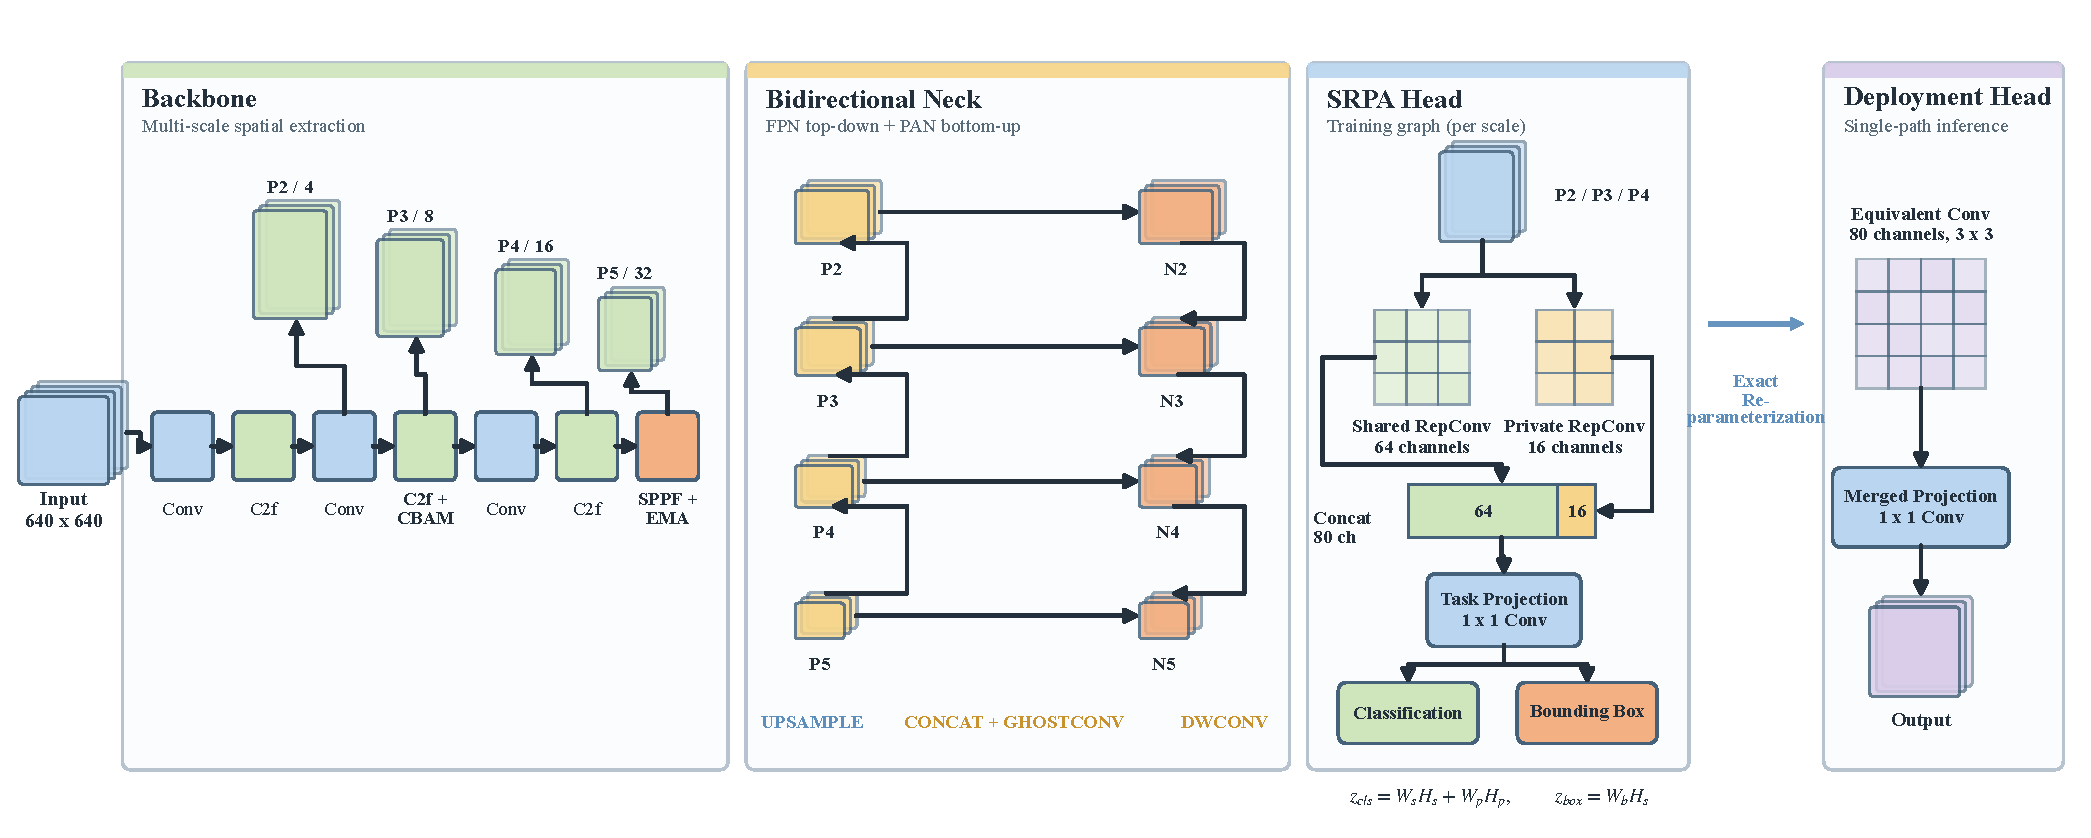
\includegraphics[width=\textwidth]{Fig1.pdf}
\caption{SRPA-YOLO 总体结构。多尺度骨干与双向颈部输出 P2--P4 特征；训练阶段分别优化共享表征和分类私有表征，精确融合后得到单路径静态部署结构。\label{fig:network}}
\end{figure*}

\subsubsection{多尺度空间特征提取}
设输入图像为 $X_0\in\mathbb{R}^{3\times640\times640}$，骨干第 $l$ 阶段输出可表示为
\begin{equation}
X_l=\mathcal{B}_l(X_{l-1})=\mathcal{A}_l\!\left(\operatorname{BN}(K_l*X_{l-1}+b_l)\right),
\label{eq:backbone}
\end{equation}
其中，$K_l$ 表示空间卷积，$\operatorname{BN}$ 表示批归一化，$\mathcal{A}_l$ 包含 SiLU 激活和局部 C2f 聚合。P2、P3、P4 与 P5 特征的步长为 $s_l\in\{4,8,16,32\}$。对于变换后最长边为 $d$ 像素的目标，其在第 $l$ 层上的近似覆盖范围为
\begin{equation}
n_l=\frac{d}{s_l}.
\label{eq:targetsupport}
\end{equation}
因此，$d=8$ 像素的无人机在 P2 上约覆盖两个特征单元，而在步长 8 的特征层上仅覆盖一个单元。保留 P2 能够提高极小目标的空间采样密度，降低目标在预测前被下采样消除的概率。

\subsubsection{轻量双向特征融合}
颈部同时执行自顶向下的语义传播和自底向上的空间聚合。相邻特征层的自顶向下特征 $T_l$ 与自底向上特征 $N_l$ 表示为
\begin{equation}
\begin{aligned}
T_l&=\psi_l\!\left(\left[X_l,\operatorname{Up}(T_{l+1})\right]\right),\\
N_l&=\eta_l\!\left(\left[T_l,\operatorname{Down}(N_{l-1})\right]\right),
\end{aligned}
\label{eq:neck}
\end{equation}
其中，$[\cdot,\cdot]$ 表示通道拼接，$\operatorname{Up}$ 为最近邻插值，$\operatorname{Down}$ 为深度步长卷积，$\psi_l$ 和 $\eta_l$ 为紧凑的 C2f/Ghost 特征混合器。自顶向下路径将深层语义传递到高分辨率特征，自底向上路径向深层补充边缘和位移信息。对于外观响应较弱、但仍具有局部空间对比的无人机，双向交换有助于同时保持语义判别性与定位敏感性。

\subsubsection{上下文感知特征校准}
高分辨率阶段执行通道与空间校准，深层阶段聚合更宽的上下文。对特征 $F$，校准响应可表示为
\begin{equation}
\begin{aligned}
\widetilde{F}&=F\odot M_c(F)\odot M_s(F),\\
M_c(F)&=\sigma\!\left(g_c(\operatorname{AvgPool}F,\operatorname{MaxPool}F)\right),\\
M_s(F)&=\sigma\!\left(g_s(\operatorname{Avg}_cF,\operatorname{Max}_cF)\right),
\end{aligned}
\label{eq:refinement}
\end{equation}
其中，$\odot$ 表示逐元素乘法，$\sigma$ 为 Sigmoid 函数，$g_c$ 和 $g_s$ 分别为轻量通道与空间变换。P2/P3 上的空间项用于抑制云层边缘、植被和建筑纹理等类无人机响应；深层上下文则扩大有效感受野，使孤立飞行目标与重复局部纹理更易区分。这些模块构成本文保留的基础特征提取器，本文的主要改进集中于预测头内部的任务容量分配。

\subsubsection{P2--P4 预测接口}
双向颈部在 $l\in\{2,3,4\}$ 输出 $N_l$，尺度投影将其映射到检测头输入空间：
\begin{equation}
\begin{aligned}
F_l&=P_l*N_l,\quad F_l\in\mathbb{R}^{C_l\times H_l\times W_l},\\
(H_l,W_l)&\in\{(160,160),(80,80),(40,40)\}.
\end{aligned}
\label{eq:headinput}
\end{equation}
三个尺度为 tiny 和 small 无人机提供密集覆盖，同时避免增加运行时 P5 预测分支。各尺度独立采用相同的 SRPA 分配方式，无需动态路由或尺度相关控制流。

\subsection{共享表征与私有秩分配}
传统共享检测头使分类与定位使用同一特征字典。SRPA 保留两任务共用的共享表征，并仅向分类分配低秩私有残差，如图~\ref{fig:allocation} 所示。

\begin{figure*}[!t]
\centering
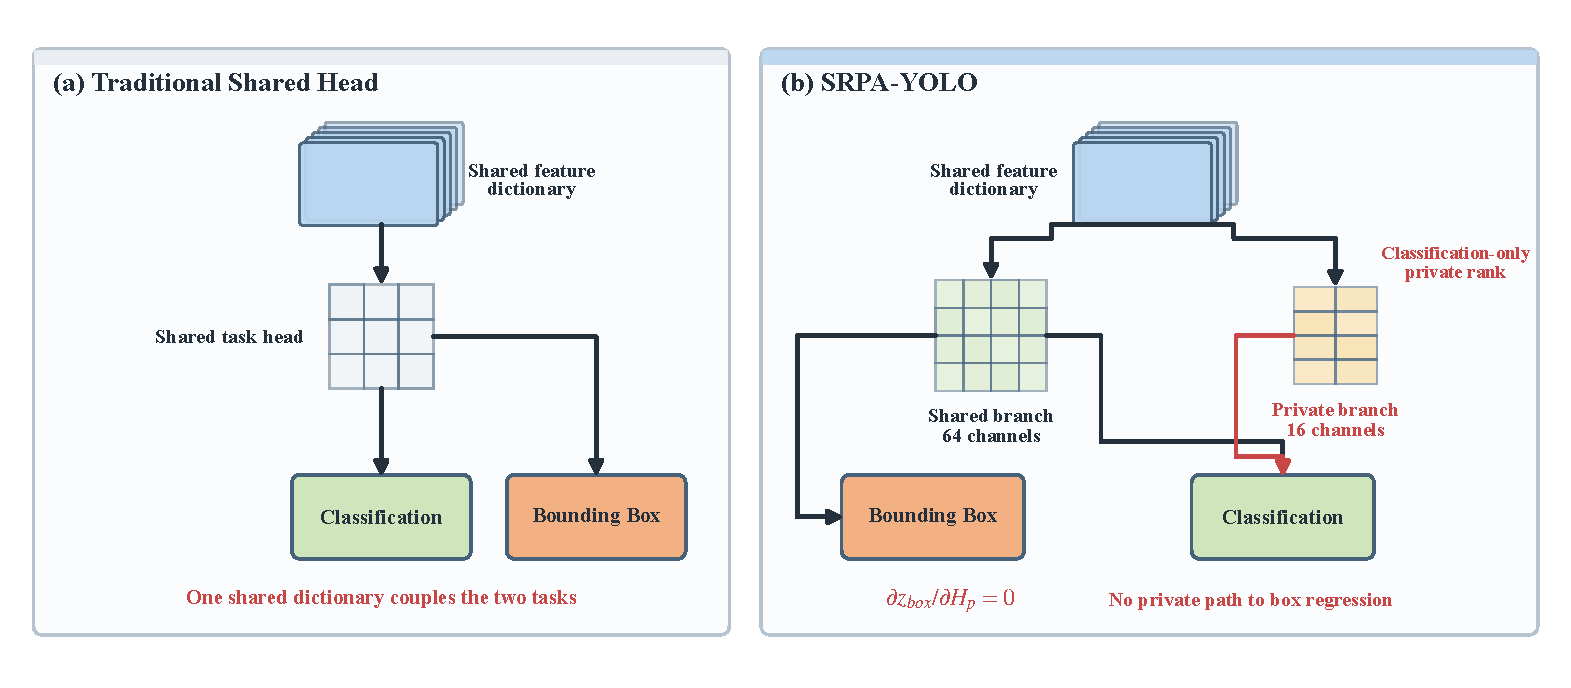
\includegraphics[width=0.92\textwidth]{Fig2.pdf}
\caption{传统共享检测头与 SRPA 检测头的任务特征分配。私有表征只参与分类，其到边界框输出的雅可比恒为零。\label{fig:allocation}}
\end{figure*}

对输入特征 $F_l$，共享 RepConv 与分类私有 RepConv 分别产生
\begin{equation}
\begin{aligned}
H_l^{s}&=\phi_s^{(l)}(F_l)\in\mathbb{R}^{64\times H_l\times W_l},\\
H_l^{p}&=\phi_p^{(l)}(F_l)\in\mathbb{R}^{16\times H_l\times W_l}.
\end{aligned}
\label{eq:features}
\end{equation}
设 $z_l^{box}$ 包含 $4K$ 个 DFL logits，且每个坐标使用 $K=16$ 个离散区间；$z_l^{cls}$ 表示无人机类别 logit。SRPA 的输出为
\begin{equation}
z_l^{box}=W_l^{b}H_l^{s}+b_l^{b},
\label{eq:box}
\end{equation}
\begin{equation}
z_l^{cls}=W_l^{s}H_l^{s}+b_l^{s}+W_l^{p}H_l^{p}.
\label{eq:cls}
\end{equation}
其中，64 和 16 通道是实现层面的表征维数，以下分别记为 $r_s$ 和 $r_p$。它们规定共享与私有通道预算，并不假设学习到的卷积矩阵必然达到满代数秩。由式~\eqref{eq:box} 和式~\eqref{eq:cls} 可得
\begin{equation}
\frac{\partial z_l^{box}}{\partial H_l^{p}}=0,
\label{eq:jacobian}
\end{equation}
该关系表明边界框输出在计算图上直接独立于分类私有表征，上游任务交互则由阶段 I 学习到的共享表征承载。将空间维展平后，$H_l^s\in\mathbb{R}^{r_s\times N_l}$、$H_l^p\in\mathbb{R}^{r_p\times N_l}$，其中 $N_l=H_lW_l$。分类 logit 的行空间满足
\begin{equation}
\begin{aligned}
z_l^{cls}-b_l^{cls}\mathbf{1}^{\top}
&\in \operatorname{row}(H_l^s)+\operatorname{row}(H_l^p),\\
\dim\!\left(\operatorname{row}(H_l^s)+\operatorname{row}(H_l^p)\right)
&\le r_s+r_p.
\end{aligned}
\label{eq:rowspace}
\end{equation}
式~\eqref{eq:rowspace} 给出组合行空间维数的上界，实际维数由各分支的学习秩及其子空间重叠共同决定。该式说明分类最多可访问 $r_s+r_p=80$ 个表征维度，而定位仅由 $r_s=64$ 个共享维度计算。私有分类投影采用 $W_l^p=0$ 初始化，并保持插入时的共享检测器不变，因此满足函数保持条件
\begin{equation}
f_{\mathrm{SRPA}}(x;W^p=0)=f_s(x),\qquad \forall x.
\label{eq:identity}
\end{equation}
扩展后的检测器以与已训练共享检测器完全一致的预测函数开始细化。私有细化期间固定骨干、颈部、共享 stem、边界框投影和共享分类投影，仅优化 $\phi_p$ 与 $W^p$。该约束使阶段 II 的既有定位映射保持不变，同时为低对比度无人机提供附加分类容量。

\FloatBarrier

\subsection{精确结构重参数化}
训练阶段的每个 RepConv stem 包含线性卷积--归一化分支。卷积核 $K$ 与批归一化参数 $(\gamma,\beta,\mu,\sigma^2)$ 可转换为
\begin{equation}
\widehat{K}=\frac{\gamma}{\sqrt{\sigma^2+\epsilon}}K,\qquad
\widehat{b}=\beta+\frac{\gamma}{\sqrt{\sigma^2+\epsilon}}(b-\mu).
\label{eq:bnfusion}
\end{equation}
将各分支卷积核补齐为 $3\times3$ 后求和。设共享和私有 stem 的等效参数分别为 $(K_s,b_s)$ 与 $(K_p,b_p)$，其中 $K_s\in\mathbb{R}^{64\times C\times3\times3}$、$K_p\in\mathbb{R}^{16\times C\times3\times3}$，则通道维精确融合为
\begin{equation}
K_d=\begin{bmatrix}K_s\\K_p\end{bmatrix},\qquad
b_d=\begin{bmatrix}b_s\\b_p\end{bmatrix}.
\label{eq:stemfuse}
\end{equation}
当 DFL 分桶数 $K=16$、类别数 $n_c=1$ 时，对应的 $1\times1$ 投影满足 $W_b\in\mathbb{R}^{4K\times64\times1\times1}$、$W_s\in\mathbb{R}^{n_c\times64\times1\times1}$ 和 $W_p\in\mathbb{R}^{n_c\times16\times1\times1}$。部署投影转换为
\begin{equation}
W_{box}^{d}=\begin{bmatrix}W_b&0\end{bmatrix},\qquad
W_{cls}^{d}=\begin{bmatrix}W_s&W_p\end{bmatrix}.
\label{eq:projfuse}
\end{equation}
对于 $H=[H_s;H_p]$，在 $W_{box}^{d}$ 的私有通道列补零可得 $W_{box}^{d}H=W_bH_s$，拼接分类投影则有 $W_{cls}^{d}H=W_sH_s+W_pH_p$。因此，每个尺度的训练期任务分解可转换为单个 80 通道 $3\times3$ 卷积和一个合并的 $1\times1$ 投影，除浮点舍入误差外计算输出不变。图~\ref{fig:reparam} 展示该过程。

\begin{figure}[!t]
\centering
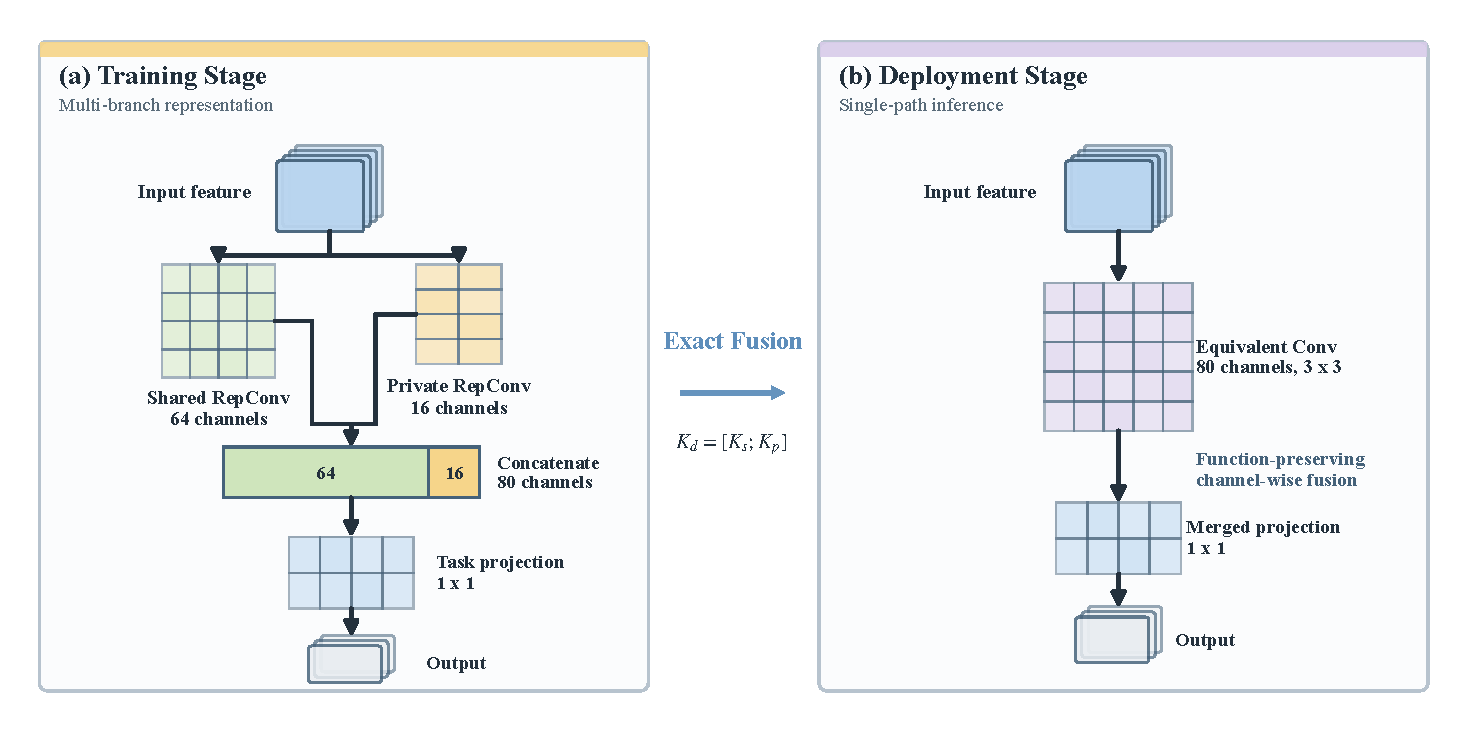
\includegraphics[width=\columnwidth]{Fig3.pdf}
\caption{SRPA 检测头的结构重参数化。并行训练表征提供任务特定容量，精确卷积核与投影融合产生单路径部署图。\label{fig:reparam}}
\end{figure}

图~\ref{fig:srpahead} 进一步展示单尺度检测头及其任务特定投影。

\begin{figure}[!t]
\centering
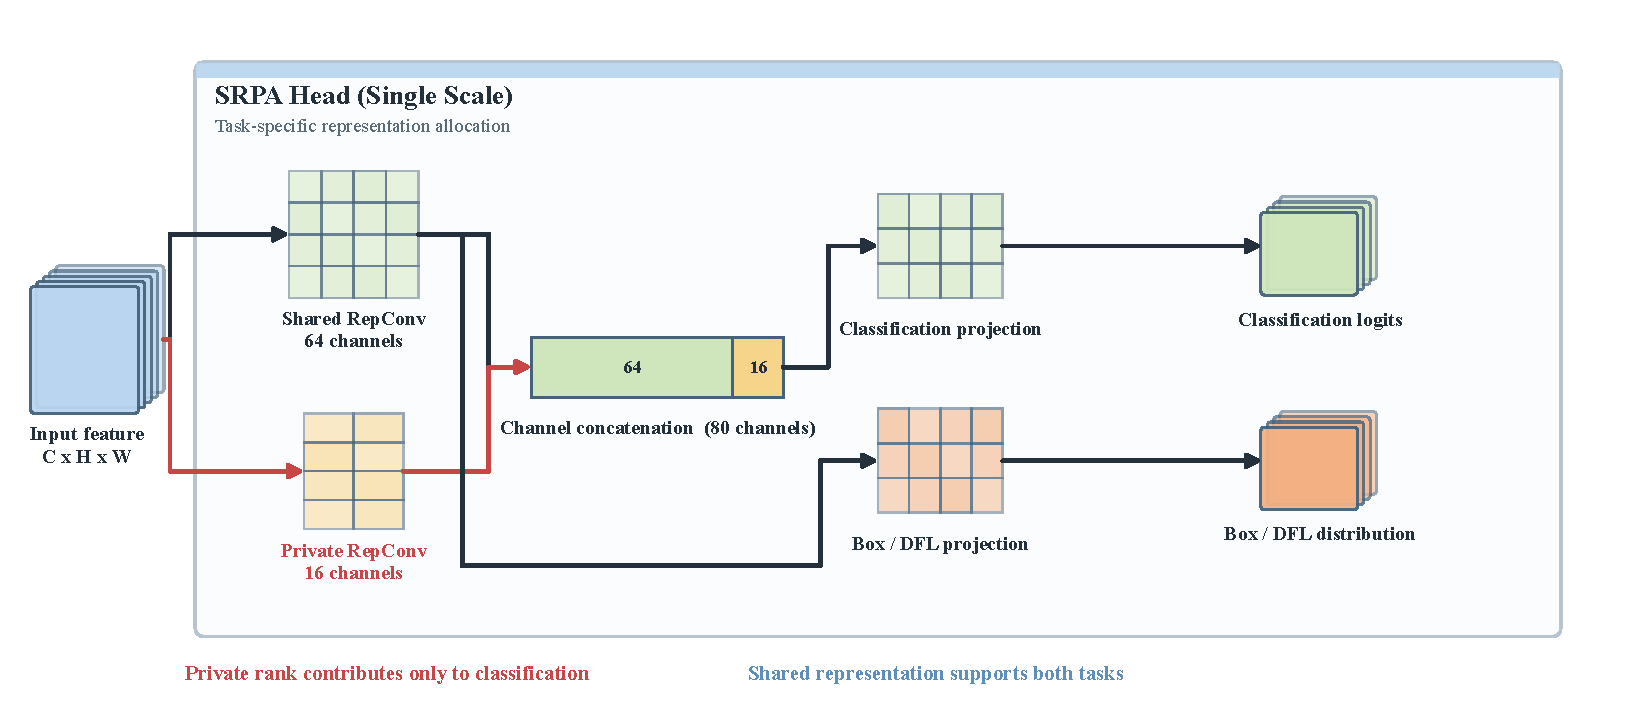
\includegraphics[width=\columnwidth]{Fig4.pdf}
\caption{SRPA 检测头内部结构。共享特征同时支持分类与定位，16 通道私有表征在部署融合前提供加性分类残差。\label{fig:srpahead}}
\end{figure}

\FloatBarrier

\subsection{目标函数与两阶段优化}
监督目标为
\begin{equation}
\begin{aligned}
\mathcal{L}_{sup}={}&\lambda_{box}\mathcal{L}_{CIoU}
+\lambda_{cls}\mathcal{L}_{BCE}
+\lambda_{dfl}\mathcal{L}_{DFL},\\
(\lambda_{box},\!\lambda_{cls},\!\lambda_{dfl})={}&(7.5,0.5,1.5),
\end{aligned}
\label{eq:sup}
\end{equation}
其中，CIoU 联合重叠率、中心距离与宽高比惩罚\cite{rezatofighi2019giou,zheng2020diou}，BCE 监督类别置信度，DFL 将每个边界框坐标表示为离散分布。

共享检测器采用冻结的 RLRD-YOLO 教师进行正则化。温度 $T=2$ 时，分类响应蒸馏为
\begin{equation}
\begin{aligned}
p_t&=\sigma(z_t^{cls}/T),\qquad p_s=\sigma(z_s^{cls}/T),\\
\mathcal{L}_{clsKD}&=T^2\operatorname{KL}(p_t\,\Vert\,p_s).
\end{aligned}
\label{eq:clskd}
\end{equation}
对正样本位置集合 $\Omega_+$，密集定位蒸馏和置信度聚焦定位蒸馏分别为
\begin{equation}
\mathcal{L}_{dflKD}=\frac{1}{N_+}\sum_{j\in\Omega_+}\operatorname{KL}\!\left(P_t^{(j)}\Vert P_s^{(j)}\right),
\label{eq:dflkd}
\end{equation}
\begin{equation}
\mathcal{L}_{focus}=\frac{\sum_{j\in\Omega_+}q_j^2\operatorname{KL}(P_t^{(j)}\Vert P_s^{(j)})}{\sum_{j\in\Omega_+}q_j^2+\epsilon},
\label{eq:focus}
\end{equation}
其中，$q_j$ 为教师置信度。阶段 I 的目标函数为
\begin{equation}
\mathcal{L}=\mathcal{L}_{sup}+0.25\mathcal{L}_{clsKD}+0.50\mathcal{L}_{dflKD}+0.125\mathcal{L}_{focus}.
\label{eq:total}
\end{equation}
阶段 II 插入零输出分类私有表征，并从式~\eqref{eq:identity} 的函数保持状态仅优化 $\phi_p$ 与 $W^p$。蒸馏过程中教师始终冻结。该训练流程先向紧凑共享检测器传递定位知识，再在阶段 II 边界框函数固定的条件下细化分类置信度。

\subsection{实验环境与训练设置}
详细训练参数见表~\ref{tab:environment}。

\begin{table}[!t]
\caption{实验环境与训练设置。\label{tab:environment}}
\centering\srpatablesetup
\begin{tabular}{@{}p{0.25\columnwidth}p{0.67\columnwidth}@{}}
\toprule
项目 & 设置\\
\midrule
框架 & Ultralytics 8.3.239 / PyTorch 2.9.0\\
CUDA & 12.8\\
GPU & NVIDIA GeForce RTX 5060，8 GB\\
输入尺寸 & $640\times640$\\
批量大小 & 32\\
训练轮数 & 200\\
优化器 & SGD\\
初始学习率 & 0.01\\
动量 & 0.937\\
权重衰减 & $5\times10^{-4}$\\
Workers & 2\\
数据增强 & HSV 抖动、水平翻转、平移、缩放、Mosaic\\
\bottomrule
\end{tabular}
\end{table}

\subsection{评价指标与部署测试}
Precision 与 Recall 定义为
\begin{equation}
P=\frac{TP}{TP+FP},\qquad R=\frac{TP}{TP+FN}.
\label{eq:pr}
\end{equation}
AP@0.50 和 AP@0.75 分别表示 IoU 阈值为 0.50 和 0.75 时 Precision--Recall 曲线下的面积。主要指标为十个阈值上的平均 AP：
\begin{equation}
\mathrm{mAP}_{0.50:0.95}=\frac{1}{10}\sum_{k=0}^{9}\mathrm{AP}_{0.50+0.05k}.
\label{eq:map}
\end{equation}
评估采用 batch size 32、置信度下限 0.001、NMS IoU 0.7，每幅图像最多保留 300 个检测结果。匹配阶段 II 实验采用随机种子 40、41 和 42，各实验使用相同的阶段 I 共享基底，并独立初始化分类私有参数，以评估私有细化过程在不同初始化条件下的性能稳定性。

共享/私有宽度分析中，设配置 $c$ 的验证集 \mapall{} 与 AP@0.75 分别为 $m_c$ 和 $a_c$。首先保留与最高验证 \mapall{} 差值不超过 0.003 的配置：
\begin{equation}
\mathcal{C}_{\epsilon}=\left\{c:m_c\ge \max_j m_j-0.003\right\},
\label{eq:selection}
\end{equation}
再选择 AP@0.75 最高的配置，若完全相同则由 AP@0.50 决定。该规则在保持主要指标的同时优先选择定位更准确的模型。

延迟测试使用 batch 1、640 像素、FP16、融合卷积、前向推理加 NMS、80 次预热和 300 次计时迭代。候选模型与 YOLOv8n 在同一进程和同一 GPU 中加载，并按 AB/BA 顺序交替测试。本文同时报告绝对延迟、FPS 和对应的同场基线结果。

\section{实验结果}

\subsection{主要精度对比}
表~\ref{tab:main} 在去重 DUT Anti-UAV 测试集上比较通用紧凑检测器与无人机专用检测器。SRPA-YOLO 的 Precision、Recall、AP@0.50、\mapall{} 和 AP@0.75 分别达到 95.850\%、92.201\%、95.185\%、67.071\% 和 77.329\%。由于 SRPA-YOLO 保留 YOLOv8 的单阶段训练与部署框架，YOLOv8n 是直接结构基线。相对 YOLOv8n，五项指标分别提高 3.088、8.242、5.057、6.895 和 9.750 个百分点，同时部署参数量减少 0.842 M。在统一评估协议下，Precision 与 Recall 同步提高，使“性能变化仅来自置信度工作点偏移”的解释可能性降低。

\begin{table*}[!t]
\caption{在 2199 张去重 DUT Anti-UAV 测试图像上的比较，粗体表示最优值。\label{tab:main}}
\centering\srpatablesetup
\begin{tabular}{lrrrrrr}\toprule
方法 & \shortstack{参数量\\(M)} & \shortstack{Precision\\(\%)} & \shortstack{Recall\\(\%)} & \shortstack{AP@0.50\\(\%)} & \shortstack{\mapall{}\\(\%)} & \shortstack{AP@0.75\\(\%)}\\\midrule
YOLO11n & 2.582 & 92.682 & 83.868 & 90.100 & 59.280 & 66.383\\
YOLOv8n & 3.006 & 92.762 & 83.959 & 90.128 & 60.176 & 67.579\\
EDGS-YOLOv8 & 3.091 & 94.266 & 83.244 & 90.428 & 60.347 & 66.415\\
DRBD-YOLOv8 & 3.047 & 92.658 & 83.601 & 90.203 & 60.689 & 67.459\\
YOLOv8n-P2 & 2.921 & \textbf{96.114} & 90.375 & 93.977 & 65.407 & 76.290\\
RLRD-YOLO & 2.926 & 95.781 & 90.107 & 94.467 & 65.436 & 74.757\\
\textbf{SRPA-YOLO} & \textbf{2.164} & 95.850 & \textbf{92.201} & \textbf{95.185} & \textbf{67.071} & \textbf{77.329}\\\midrule
$\Delta$ SRPA 相对 YOLOv8n & $-0.842$ & $+3.088$ & $+8.242$ & $+5.057$ & $+6.895$ & $+9.750$\\\bottomrule
\end{tabular}
\end{table*}


图~\ref{fig:comparison} 汇总各检测器的精度与紧凑性对比。

\begin{figure*}[!t]
\centering
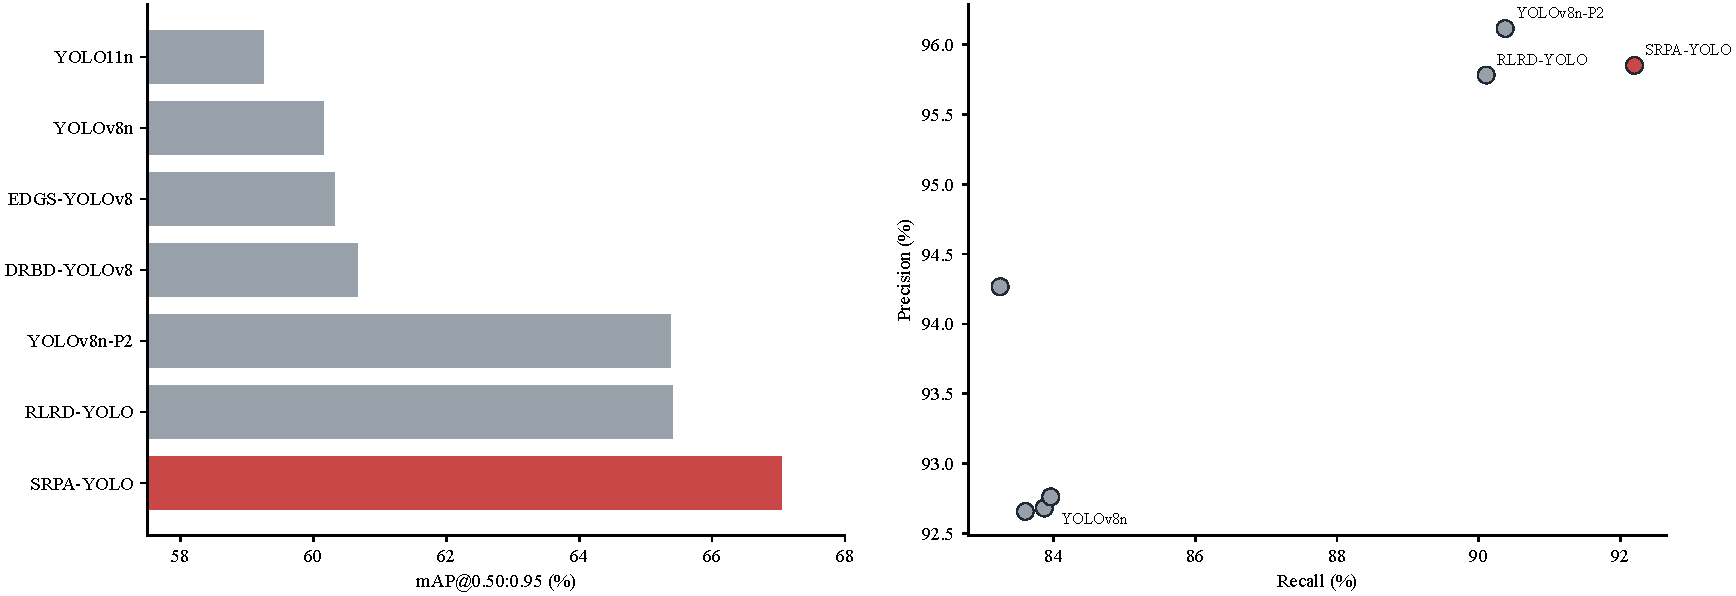
\includegraphics[width=\textwidth]{Fig5.pdf}
\caption{去重 DUT Anti-UAV 测试集上的精度与紧凑性对比，检测指标均采用百分制。\label{fig:comparison}}
\end{figure*}

YOLOv8n-P2 用于控制高分辨率预测层带来的影响。尽管其 Precision 高 0.264 个百分点，SRPA-YOLO 的 Recall、AP@0.50、\mapall{} 和 AP@0.75 仍分别提高 1.826、1.208、1.664 和 1.039 个百分点。该对比表明，检测头任务特征分配在高分辨率尺度扩展之外仍能带来进一步增益。

图~\ref{fig:complexity} 展示部署参数量与 \mapall{} 的关系。SRPA-YOLO 位于左上区域，在对比模型中同时获得最高 \mapall{} 和最小参数量。该工作点与“使用紧凑共享字典，并仅向分类分配附加容量”的设计目标一致。

\begin{figure}[!t]
\centering
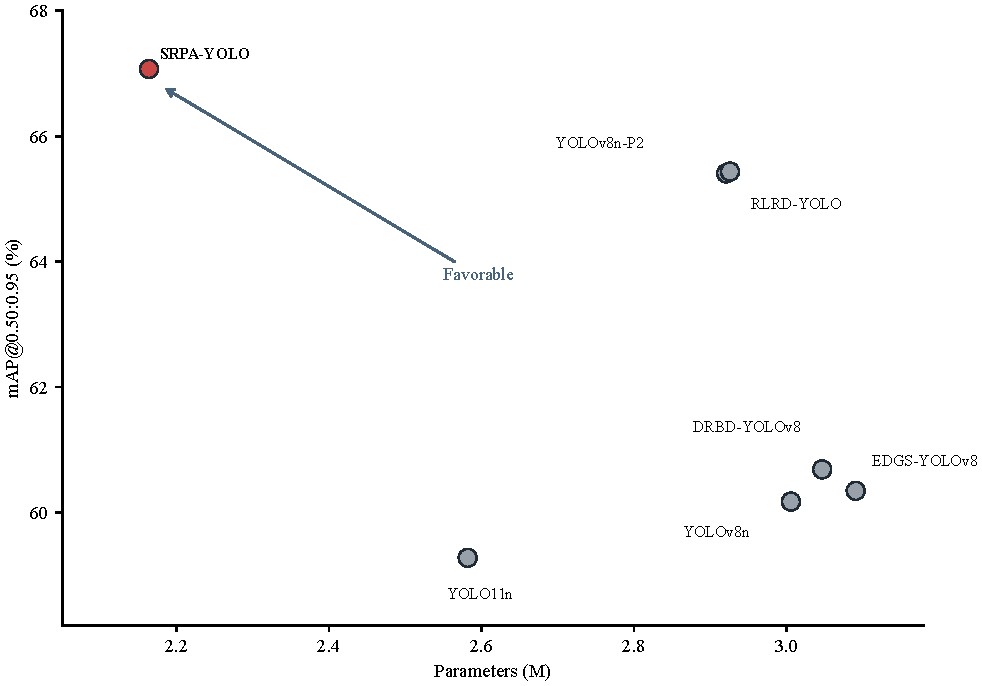
\includegraphics[width=\columnwidth]{Fig6.pdf}
\caption{模型复杂度权衡。横轴为部署参数量，纵轴为 \mapall{}，箭头表示更优方向。\label{fig:complexity}}
\end{figure}

\subsection{共享/私有秩与机制消融}
表~\ref{tab:rank} 在验证集上独立分析共享秩与私有秩。共享秩从 48 增至 64 或 80 时，\mapall{} 并未单调增加，说明统一增宽不足以确定最优配置。48+16 取得最高验证 \mapall{}（60.874\%），64+16 则取得最高 AP@0.75（69.986\%）、AP@0.50（91.850\%）和 Precision（96.615\%）。依据式~\eqref{eq:selection}，两种分配均处于最高 \mapall{} 的 0.3 个百分点内，64+16 因具有更强的高 IoU 定位性能而被选用。

\begin{table*}[!t]
\caption{共享秩与私有秩的验证集消融。\label{tab:rank}}
\centering\srpatablesetup
\begin{tabular}{rrrrrrr}\toprule
$r_s$ & $r_p$ & \shortstack{参数量\\(M)} & \shortstack{P\\(\%)} & \shortstack{R\\(\%)} & \shortstack{AP@0.50\\(\%)} & \shortstack{\mapall{}/\\AP@0.75 (\%)}\\\midrule
48 & 0  & 2.093 & 96.089 & 87.182 & 91.667 & 60.508 / 69.337\\
64 & 0  & 2.128 & 96.378 & 86.570 & 91.703 & 60.454 / 69.754\\
80 & 0  & 2.164 & 96.073 & \textbf{87.743} & 91.569 & 60.513 / 69.262\\
48 & 16 & 2.128 & 96.135 & 87.310 & 91.798 & \textbf{60.874} / 69.618\\
\textbf{64} & \textbf{16} & \textbf{2.164} & \textbf{96.615} & 86.570 & \textbf{91.850} & 60.646 / \textbf{69.986}\\\bottomrule
\end{tabular}
\end{table*}


表~\ref{tab:mechanism} 展示从完整非线性检测头到最终 SRPA 配置的累积变化。加入密集 DFL 蒸馏与检测头压缩精度的恢复相关，随后增加的置信度聚焦项对应 0.384 个 \mapall{} 百分点增量。在累积协议下，迁移初始化对应 Recall 和 \mapall{} 分别提高 2.660 和 0.678 个百分点；共享表征增至 64 通道后，\mapall{} 和 AP@0.75 分别增加 0.531 和 1.674 个百分点。最终，16 通道分类私有残差使 \mapall{} 达到 67.071\%，AP@0.75 达到 77.329\%。各行均保留前序组件，并报告相应累积配置的性能。共享 80 通道对照获得相近的 67.121\% \mapall{}，而 64+16 分配还满足式~\eqref{eq:jacobian} 的零边界框雅可比，并由预先定义的验证集定位准则选出。结合秩消融，结果支持受任务约束的容量分配优于不受约束的检测头增宽。

\begin{table*}[!t]
\caption{去重 DUT Anti-UAV 测试集上的机制消融。\label{tab:mechanism}}
\centering\srpatablesetup
\begin{tabular}{p{0.27\textwidth}rrrrrr}\toprule
配置 & \shortstack{参数量\\(M)} & \shortstack{P\\(\%)} & \shortstack{R\\(\%)} & \shortstack{AP@0.50\\(\%)} & \shortstack{\mapall{}\\(\%)} & \shortstack{AP@0.75\\(\%)}\\\midrule
完整非线性头 & 2.603 & 95.922 & 90.954 & 94.736 & 66.046 & 75.503\\
Shared-48 + 密集 DFL KD & 2.093 & 96.152 & 90.954 & 94.836 & 65.363 & 74.929\\
$+$ 聚焦定位 KD & 2.093 & 97.084 & 90.285 & 95.018 & 65.747 & 75.573\\
$+$ 高容量初始化迁移 & 2.093 & 96.484 & 92.945 & \textbf{95.493} & 66.425 & 75.472\\
$+$ 共享秩 64 & 2.128 & 96.122 & 92.157 & 95.366 & 66.956 & 77.146\\
$+$ 私有秩 16 & 2.164 & 95.850 & 92.201 & 95.185 & \textbf{67.071} & \textbf{77.329}\\\bottomrule
\end{tabular}
\end{table*}


\subsection{定位与尺度特性}
图~\ref{fig:scaleiou} 在 0.50--0.95 的 IoU 阈值范围内直接比较 SRPA-YOLO 与 YOLOv8n。SRPA-YOLO 在每个阈值上均取得更高 AP：IoU 0.50 时差值为 5.057 个百分点，IoU 0.75 时增至 9.750 个百分点，IoU 0.85 时仍为 8.803 个百分点。严格重叠条件下仍保持优势，说明实测改进包含定位因素，而不局限于 IoU 0.50 下的分类置信度变化。

\begin{figure*}[!t]
\centering
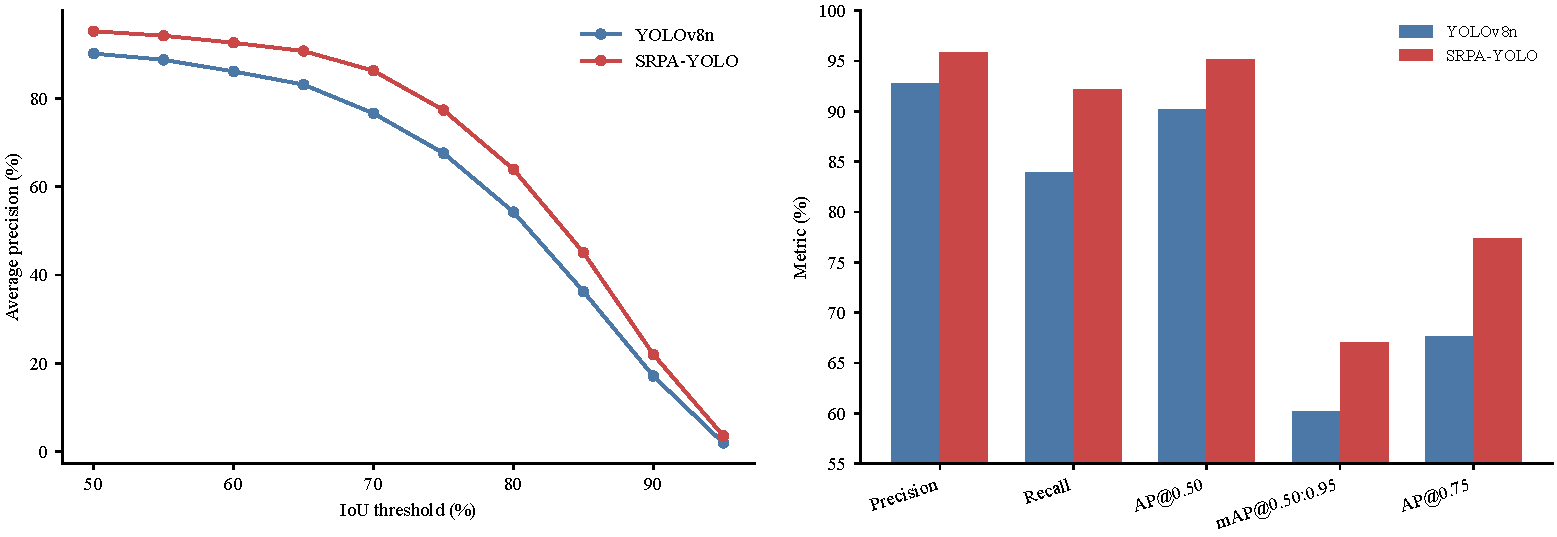
\includegraphics[width=0.96\textwidth]{Fig7.pdf}
\caption{SRPA-YOLO 与 YOLOv8n 的定位对比。左：各 IoU 阈值下的 AP；右：综合检测指标。\label{fig:scaleiou}}
\end{figure*}

相对 YOLOv8n，最大的综合提升出现在 Recall（+8.242 个百分点），同时 AP@0.50 和 AP@0.75 均增加。在远距离无人机监测中，更高 Recall 可直接减少漏检，而 Precision 的同步提升限制了附加误警。P2 预测层为 tiny 无人机提供空间支撑，SRPA 检测头则使分类私有细化不进入边界框回归输入。该结构解释与低、高 IoU 阈值下的实测增益一致。

\subsection{定性检测分析}
图~\ref{fig:detectioncomparison} 在置信度阈值为 0.25 时，对相同 tiny UAV 实例上的 YOLOv8n 与 SRPA-YOLO 检测结果进行比较。当预测框与真值框的 IoU 不低于 0.50 时，将其判定为正确检测。三个所选样例中，YOLOv8n 均未产生满足匹配条件的预测，而 SRPA-YOLO 能够恢复目标。这些代表性案例从视觉层面印证了测试集定量指标所反映的性能提升；局部放大图展示了所恢复预测与仅占少量像素目标的空间对齐情况。

\begin{figure*}[!t]
\centering
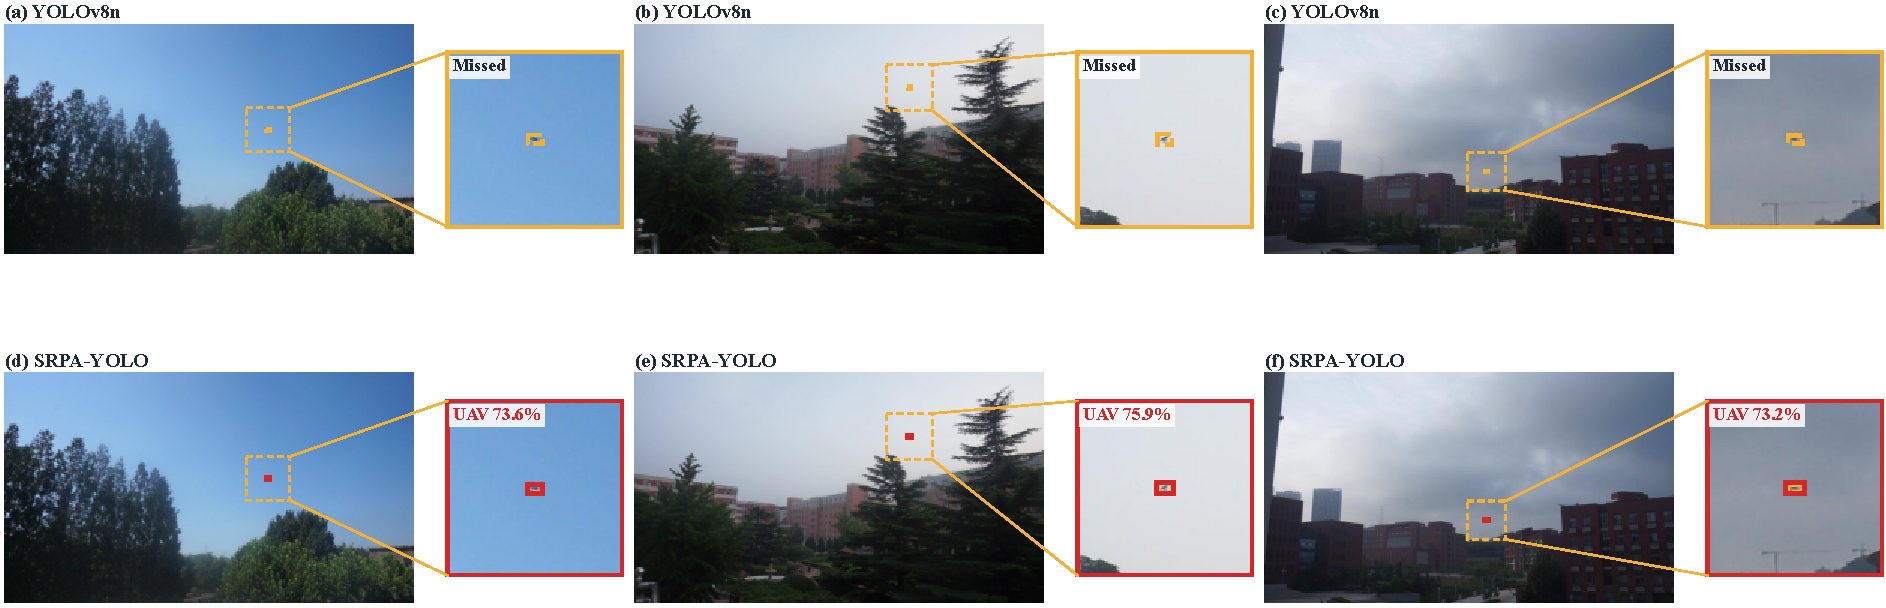
\includegraphics[width=\textwidth]{Fig8.pdf}
\caption{去重 DUT Anti-UAV 测试集上的同图检测对比。黄色虚线框表示真值，红色实线框表示 SRPA-YOLO 预测；“Missed”表示 YOLOv8n 不存在同时满足置信度 $\geq0.25$ 和 IoU $\geq0.50$ 的预测。\label{fig:detectioncomparison}}
\end{figure*}

图~\ref{fig:tinydetections} 进一步展示 SRPA-YOLO 在天空、建筑、植被和低对比度背景中的成功检测结果。所选目标经 640 像素 letterbox 变换后的最长边仅为 5.7--6.3 px。尽管目标空间支撑有限且背景占比很高，保留的 checkpoint 在各所选场景中均形成了定位响应。这些案例直观展示了模型在天空、植被、建筑和低对比度背景中的小目标检测能力，并与前述测试集指标保持一致。

\begin{figure*}[!t]
\centering
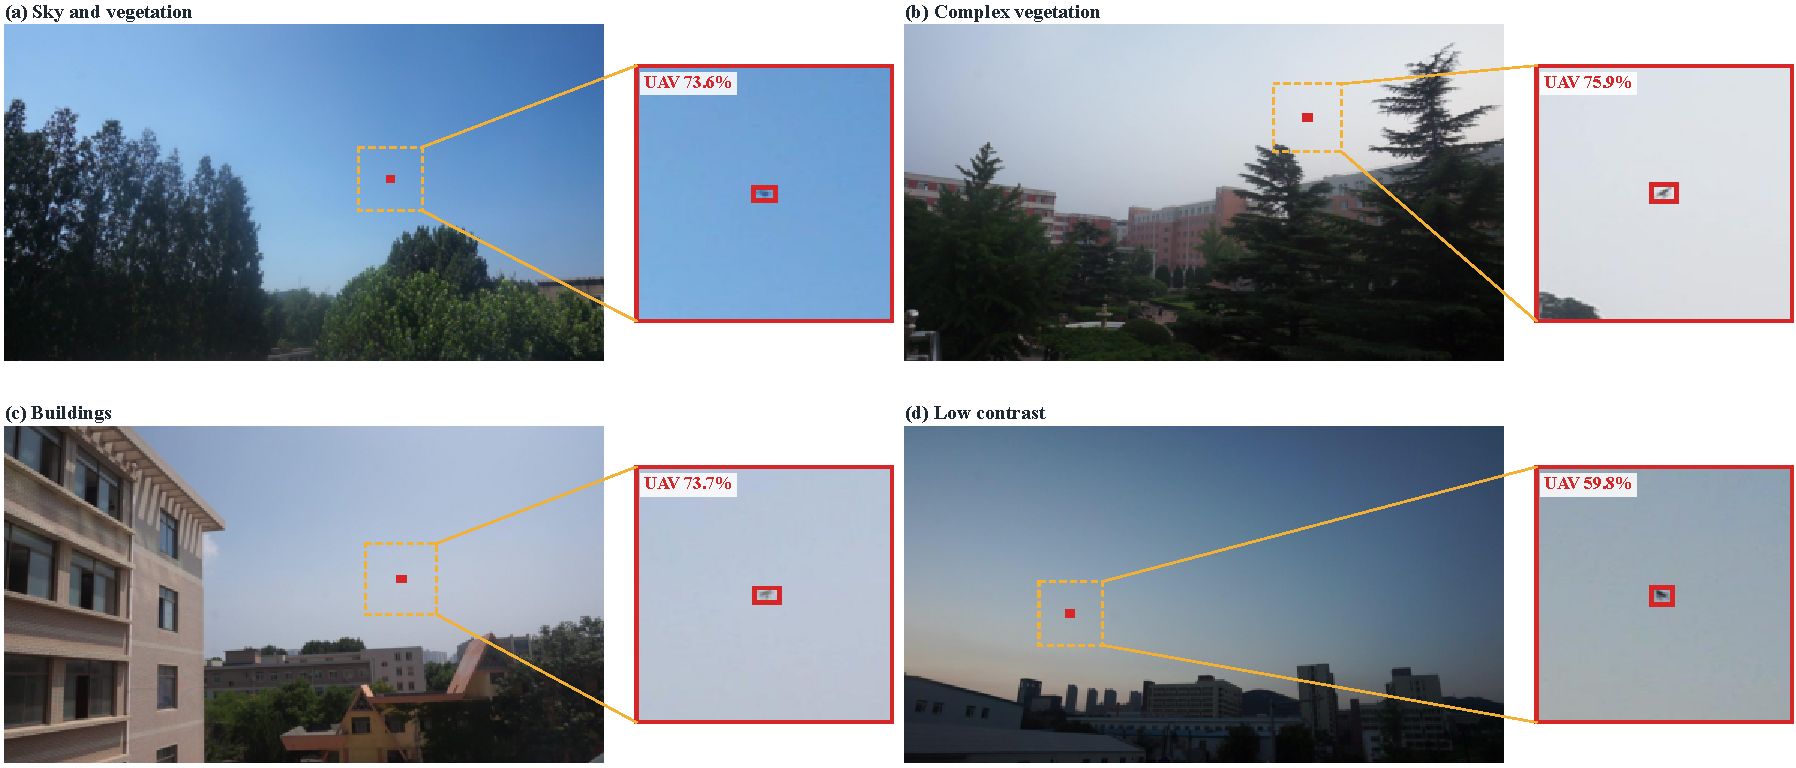
\includegraphics[width=0.90\textwidth]{Fig9.pdf}
\caption{SRPA-YOLO 对 tiny UAV 的成功检测结果。每组右侧区域为对应原图中的目标局部放大，红色框和标签来自最终保留 checkpoint 的预测。\label{fig:tinydetections}}
\end{figure*}

\subsection{匹配随机种子稳定性}
表~\ref{tab:seeds} 汇总了阶段 II 随机种子 40、41 和 42 的实验结果。各实验采用相同的阶段 I 共享基底，并独立初始化分类私有参数。SRPA-YOLO 的 Recall、AP@0.50 和 \mapall{} 标准差分别为 0.112、0.022 和 0.082 个百分点，表明分类私有细化在不同初始化条件下保持了较低的性能波动。相对 RLRD-YOLO，Recall、\mapall{} 和 AP@0.75 的平均配对提升分别为 2.709、1.881 和 2.150 个百分点，说明所提出的分类私有表征能够在多个匹配种子下持续改善检测精度。

\begin{table*}[!t]
\caption{三个匹配阶段 II 随机种子在去重 DUT Anti-UAV 测试集上的均值与样本标准差（\%，$n=3$）。各实验使用相同的阶段 I 共享基底，仅独立初始化私有参数。\label{tab:seeds}}
\centering\srpatablesetup
\begin{tabular}{lrrrrr}\toprule
方法 & \shortstack{Precision\\(\%)} & \shortstack{Recall\\(\%)} & \shortstack{AP@0.50\\(\%)} & \shortstack{\mapall{}\\(\%)} & \shortstack{AP@0.75\\(\%)}\\\midrule
RLRD-YOLO & $95.964\pm0.766$ & $89.463\pm0.785$ & $94.661\pm0.106$ & $65.199\pm0.639$ & $75.196\pm0.564$\\
SRPA-YOLO & $96.167\pm0.031$ & $92.172\pm0.112$ & $95.304\pm0.022$ & $67.080\pm0.082$ & $77.345\pm0.233$\\
配对差值 & $+0.204\pm0.736$ & $+2.709\pm0.773$ & $+0.644\pm0.109$ & $+1.881\pm0.721$ & $+2.150\pm0.332$\\\bottomrule
\end{tabular}
\end{table*}


\subsection{延迟与部署复杂度}
训练图约含 2.18 M 参数，在 640 像素输入下为 8.5 GFLOPs。结构融合移除训练期状态后，部署 checkpoint 含 2.164 M 参数。表~\ref{tab:latency} 给出同进程配对测试，其中每个检测器均与同场 YOLOv8n 对照共同测量；表~\ref{tab:cleanlat} 给出独立低负载最终验收结果。

\begin{table*}[!t]\caption{同进程配对延迟。batch 1、640、FP16、融合前向+NMS、80 次预热、300 次计时；Control 为同步 YOLOv8n。\label{tab:latency}}\centering\srpatablesetup
\begin{tabular}{lrrrrrr}\toprule
&\multicolumn{3}{c}{第1轮}&\multicolumn{3}{c}{第2轮}\\\cmidrule(lr){2-4}\cmidrule(lr){5-7}
方法&ms&FPS&Control ms&ms&FPS&Control ms\\\midrule
YOLO11n&21.6357&46.22&16.8632&19.1505&52.22&15.0139\\
YOLOv8n-P2&19.1953&52.10&15.9227&16.9629&58.95&14.1962\\
EDGS*&19.5146&51.24&14.6088&22.0043&45.45&16.3604\\
DRBD*&29.0158&34.46&14.5733&31.7115&31.53&16.8584\\
RLRD-YOLO&22.5644&44.32&16.0771&22.7773&43.90&16.2647\\
\textbf{SRPA-YOLO}&\textbf{16.2469}&\textbf{61.55}&16.4922&\textbf{15.0936}&\textbf{66.25}&15.5909\\\bottomrule
\end{tabular}\end{table*}
\begin{table*}[!t]\caption{SRPA-YOLO 与同场 YOLOv8n 对照在相同 batch 1、640 像素、FP16、融合前向+NMS 协议下的独立低负载最终验收结果。\label{tab:cleanlat}}\centering\srpatablesetup
\begin{tabular}{lrrrr}\toprule
轮次&SRPA-YOLO(ms)&SRPA-YOLO(FPS)&YOLOv8n(ms)&YOLOv8n(FPS)\\\midrule
1&9.7435&102.63&9.8859&101.15\\2&9.8574&101.45&9.9893&100.11\\\bottomrule
\end{tabular}\end{table*}


在另一组低负载验收测试中，SRPA-YOLO 两轮延迟为 9.7435 和 9.8574 ms（102.63 和 101.45 FPS），同场测量的 YOLOv8n 对照为 9.8859 和 9.9893 ms（101.15 和 100.11 FPS）。二者两轮均值分别为 9.8005 和 9.9376 ms。在所报告的配对测试协议下，SRPA-YOLO 在保持相当帧时间的同时，将部署参数量减少了 28.0\%。

图~\ref{fig:speedtradeoff} 展示所报告的两轮平均延迟与主要精度指标之间的关系。在已测模型和当前硬件协议范围内，SRPA-YOLO 位于有利的精度--速度边界：精度相近的模型具有更高实测延迟，而更快的模型未达到相同 \mapall{}。

\begin{figure}[!t]
\centering
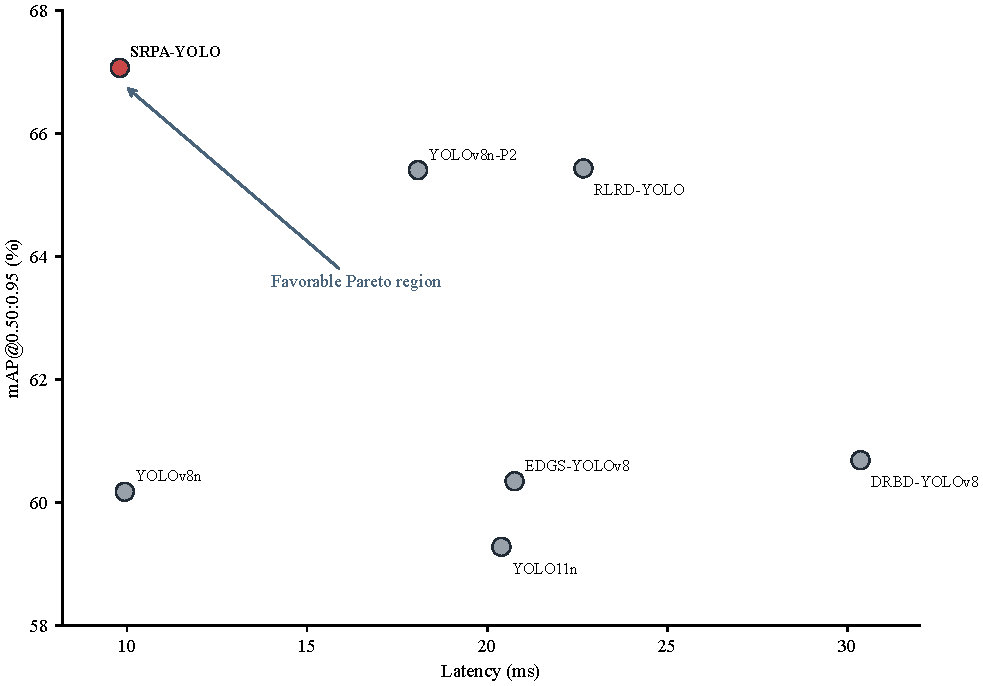
\includegraphics[width=0.78\columnwidth]{Fig10.pdf}
\caption{基于两轮平均延迟与 \mapall{} 的精度--速度权衡，SRPA-YOLO 位于有利 Pareto 区域。\label{fig:speedtradeoff}}
\end{figure}

\section{结论}

本文提出 SRPA-YOLO，将预测头容量表述为任务特定的表征分配问题。64 通道共享表征同时支持分类与 DFL 定位，零输出初始化的 16 通道分类私有表征仅提供加性分类残差。该结构扩展分类可用的特征容量，并使边界框输出在计算图上直接独立于私有表征。精确结构重参数化将训练期分解转换为每尺度一个 80 通道卷积和一个合并输出投影，形成静态单路径部署图。

在去重 DUT Anti-UAV 测试集上，验证集选出的 checkpoint 取得 95.850\% Precision、92.201\% Recall、95.185\% AP@0.50、67.071\% \mapall{} 和 77.329\% AP@0.75，部署参数量为 2.164 M。相对 YOLOv8n，五项指标分别提高 3.088、8.242、5.057、6.895 和 9.750 个百分点，同时参数量减少 28.0\%。相对 YOLOv8n-P2，SRPA-YOLO 的 Recall、AP@0.50、\mapall{} 和 AP@0.75 进一步提高，表明检测头任务分配与高分辨率预测具有互补作用。各 IoU 阈值下的一致精度优势以及匹配随机种子实验中的较低性能波动，进一步体现了 SRPA-YOLO 在定位与分类细化方面的稳定表现。

在规定的 RTX 5060、FP16、batch 1、前向推理加 NMS 协议下，SRPA-YOLO 两轮配对延迟为 9.7435 和 9.8574 ms，YOLOv8n 为 9.8859 和 9.9893 ms。结合 28.0\% 的参数量缩减，这些结果表明 SRPA-YOLO 在所评估 GPU 软件栈上获得了有利的精度--紧凑性工作点。后续研究将扩展至多类别航拍场景、更多数据集、嵌入式 ONNX/TensorRT 部署，并分析尺度条件私有容量在不同目标尺度分布下的静态融合性质。

\section*{声明}

\noindent\textbf{资金支持。} 作者声明，本研究在论文准备过程中未获得任何资金、基金或其他外部资助。

\noindent\textbf{利益冲突。} 作者声明不存在与本研究相关的财务或非财务利益冲突。

\noindent\textbf{作者贡献。} 王显普：研究构思、方法设计、软件实现、验证、形式分析、调查、数据整理、可视化和初稿撰写。职海杰：验证、形式分析和论文审阅与修改。费庆：研究构思、监督、资源、项目管理和论文审阅与修改。所有作者均已阅读并同意论文最终版本。

\noindent\textbf{数据与代码可用性。} DUT Anti-UAV 数据集可依据数据提供方条款从其公开项目获取。复现包包含去重清单、源代码、模型配置、结果清单、配对延迟记录和可编辑绘图脚本。上述材料与训练权重可向通信作者获取，并将存入带版本号的公共仓库。固定评估清单排除一项跨数据划分重复样本，并记录其 SHA-256 哈希；源图像均未删除。

\begin{acknowledgements}
作者感谢 DUT Anti-UAV 基准和 Ultralytics 开源框架的维护者。
\end{acknowledgements}


\bibliographystyle{spmpsci}
\bibliography{../bibliography/references}

\end{document}
